\subsection{The CheXFound Vision Foundation Model and ViT Architecture}
\label{subsec:chexfound_vit}

To address the limitations of centralized and domain-restricted architectures under severe data siloing, modern clinical pipelines are shifting toward Vision Foundation Models (VFMs). At the forefront of this shift is \textbf{CheXFound}, a self-supervised, vision-centric foundation model engineered explicitly for high-throughput, multi-class thoracic imaging diagnosis. CheXFound eliminates the historical constraint of training standalone networks for separate diagnostic indications by building generalized, highly robust chest representations. By utilizing a heavy Vision Transformer (ViT) architecture rather than a conventional convolutional backbone, CheXFound effectively captures long-range dependencies, contextual anatomical relationships, and fine-grained pathological variations across heterogeneous image streams.

\subsubsection{The Vision Transformer (ViT-Large) Backbone Architecture}

CheXFound is structurally built upon a modified \textbf{ViT-Large (ViT-L/16)} structural spine, optimizing representation capabilities at an expanded spatial resolution of $512\times512$ pixels. This configuration is mathematically designed to process image grids without losing subtle pathological signals, such as micro-nodular patterns or faint ground-glass borders, which often disappear when compressed into lower-resolution latent matrices. 

The structural flow of the forward pass within CheXFound's ViT-L/16 architecture proceeds as follows:

\begin{enumerate}
	\item \textbf{Patch Extraction and Flattening:} A continuous two-dimensional input thoracic image $\mathbf{X} \in \mathbb{R}^{H \times W \times C}$ (where $H=W=512$ and $C=1$ for radiographs or single-slice CTs) is systematically split into a grid of non-overlapping, uniform rectangular patches $\mathbf{X}_p \in \mathbb{R}^{N \times (P^2 \cdot C)}$. Here, $P = 16$ denotes the hardcoded spatial patch size, and $N$ represents the resulting total number of sequence patches, computed mathematically as:
	\begin{equation}
		N = \frac{H \cdot W}{P^2} = \frac{512 \times 512}{16 \times 16} = 1024 \text{ patches}
	\end{equation}
	
	\item \textbf{Linear Patch Embedding:} Each flattened structural patch token is projected into a lower-dimensional latent embedding space using a trainable linear mapping matrix $\mathbf{E} \in \mathbb{R}^{(P^2 \cdot C) \times D}$, where $D = 1024$ defines the dense hidden embedding dimension of the ViT-Large backbone.
	
	\item \textbf{CLS Token Prepended and Position Encodings:} A learnable classification token embedding $\mathbf{z}_0^0 = \mathbf{x}_{\text{class}} \in \mathbb{R}^D$ is prepended to the sequence of patch tokens. To preserve the two-dimensional spatial topography of the chest inside a one-dimensional sequence pipeline, standard learnable one-dimensional position encodings $\mathbf{E}_{\text{pos}} \in \mathbb{R}^{(N+1) \times D}$ are element-wise added to the patch embeddings, yielding the initial input tensor $\mathbf{z}_0$:
	\begin{equation}
		\mathbf{z}_0 = \left[ \mathbf{x}_{\text{class}}; \, \mathbf{X}_p^1\mathbf{E}; \, \mathbf{X}_p^2\mathbf{E}; \, \dots; \, \mathbf{X}_p^N\mathbf{E} \right] + \mathbf{E}_{\text{pos}}
	\end{equation}
	
	\item \textbf{Transformer Encoder Blocks:} The combined sequence $\mathbf{z}_0$ passes sequentially through $L = 24$ identical Transformer Encoder blocks. Each block features a Multi-Head Self-Attention (\text{MHSA}) mechanism with $h = 16$ distinct attention heads, interleaved with Multi-Layer Perceptron (\text{MLP}) blocks and scaled by Layer Normalization (\text{LN}) using residual skip-connections:
	\begin{align}
		\mathbf{z}_{\ell}' &= \text{MHSA}(\text{LN}(\mathbf{z}_{\ell-1})) + \mathbf{z}_{\ell-1}, \quad \ell = 1, \dots, 24 \\
		\mathbf{z}_{\ell} &= \text{MLP}(\text{LN}(\mathbf{z}_{\ell}')) + \mathbf{z}_{\ell}'
	\end{align}
\end{enumerate}

The standard ViT core configuration embedded inside CheXFound is mathematically mapped and detailed in Table~\ref{tab:vit_large_specs}.

\begin{table}[htbp]
	\centering
	\caption{Structural and mathematical parameter configurations of the CheXFound ViT-Large/16 backbone layout.}
	\label{tab:vit_large_specs}
	\small
	\begin{tabularx}{\textwidth}{lXX}
		\toprule
		\textbf{Architectural Hyperparameter} & \textbf{Formal Definition / Notation} & \textbf{Deterministic Global Value} \\
		\midrule
		\textbf{Input Resolution} & $H \times W \times C$ & $512 \times 512 \times 1$ Pixels \\
		\addlinespace
		\textbf{Patch Dimension} & $P \times P$ & $16 \times 16$ Pixels \\
		\addlinespace
		\textbf{Sequence Count} & $N = (H \cdot W)/P^2$ & $1024$ Active Patch Tokens \\
		\addlinespace
		\textbf{Hidden Layer Dimension} & $D$ & $1024$ Scaled Scaling Dimensions \\
		\addlinespace
		\textbf{Transformer Layers} & $L$ & $24$ Cascaded Encoder Blocks \\
		\addlinespace
		\textbf{Attention Heads} & $h$ & $16$ Independent Heads \\
		\addlinespace
		\textbf{MLP Expansion Ratio} & $\text{Ratio}_{\text{MLP}}$ & $4.0 \times D$ ($4096$ Hidden Units) \\
		\bottomrule
	\end{tabularx}
\end{table}

\subsubsection{Pretraining Paradigm and Self-Supervised Objective Functions}

CheXFound is pretrained on a curated, large-scale medical dataset comprising approximately 987,000 unique chest radiographs derived from 12 distinct open-source clinical databases (including MIMIC-CXR, CheXpert, PadChest, and BraX). To extract optimal task-agnostic representations without relying on manual labels, CheXFound utilizes the **DINOv2** self-supervised learning pipeline. This setup combines a student network (parameterized by weights $\theta_s$) and a teacher network (parameterized by weights $\theta_t$). The teacher's weights are updated continuously via an Exponential Moving Average (EMA) of the student's weights:
\begin{equation}
	\theta_t \leftarrow \lambda \theta_t + (1 - \lambda)\theta_s
\end{equation}

The optimization function combines a multi-crop global-to-local cross-entropy loss with an explicit Masked Image Modeling (MIM) autoencoder objective function. Given a global view image input $x_g$ and a local masked crop input $x_l$, the multi-crop cross-entropy loss enforces representational consistency across scales:
\begin{equation}
	\mathcal{L}_{\text{global}} = \sum_{x \in \{x_g, x_l\}} \sum_{i \neq j} H\left(P_t(x^{(i)}), P_s(x^{(j)})\right)
\end{equation}
where $H(p, q) = -p \log q$, and $P_t, P_s$ denote the soft probability outputs generated by passing the $\mathbf{x}_{\text{class}}$ token through a centering and sharpening bottleneck.

Concurrently, the MIM objective function randomly masks out a subset of the patch sequence tokens (typically 50\% bounding ratios) before feeding them into the student network. The model then computes a localized categorical cross-entropy loss at the patch-token level against the unmasked teacher representations, training the model to predict contextual structure:
\begin{equation}
	\mathcal{L}_{\text{MIM}} = -\sum_{k \in \mathcal{M}} P_t(\mathbf{z}_k) \log P_s(\mathbf{z}_k)
\end{equation}
where $\mathcal{M}$ signifies the set of index fields tracking the masked patches. The unified self-supervised optimization equation for the foundation layer is structured as:
\begin{equation}
	\mathcal{L}_{\text{CheXFound}} = \alpha \mathcal{L}_{\text{global}} + \beta \mathcal{L}_{\text{MIM}}
\end{equation}

\subsubsection{Global and Local Representations Integration (GLoRI) Downstream Adaptation Head}

Standard foundation models often lose small-scale, localized pathological indicators—such as early-stage lung cancer nodules or subtle tuberculous cavities—during global attention pooling over the classification token ($\mathbf{x}_{\text{class}}$). To prevent this loss, CheXFound introduces a specialized downstream adaptation module called the **Global and Local Representations Integration (GLoRI)** head. 

Instead of relying solely on the final layer's $\mathbf{x}_{\text{class}}$ token, the GLoRI module processes both coarse-grained global features and fine-grained, localized patch tokens. During downstream fine-tuning, the backbone CheXFound parameters remain completely frozen to preserve generalizability, while the GLoRI head operates as a trainable multi-head cross-attention layer.

The mathematical routing within the GLoRI module follows this pipeline:
\begin{enumerate}
	\item The global representation vector $\mathbf{f}_g \in \mathbb{R}^D$ is isolated from the class token $\mathbf{x}_{\text{class}}$.
	\item The array of patch tokens $\mathbf{F}_p = [\mathbf{z}_1, \mathbf{z}_2, \dots, \mathbf{z}_1024] \in \mathbb{R}^{1024 \times D}$ is mapped to extract high-resolution localized profiles.
	\item A specific cross-attention layer treats the global feature vector as the query vector ($\mathbf{Q}$), while mapping the patch tokens to generate the keys ($\mathbf{K}$) and values ($\mathbf{V}$):
	\begin{equation}
		\mathbf{Q} = \mathbf{f}_g \mathbf{W}_Q, \quad \mathbf{K} = \mathbf{F}_p \mathbf{W}_K, \quad \mathbf{V} = \mathbf{F}_p \mathbf{W}_V
	\end{equation}
	where $\mathbf{W}_Q, \mathbf{W}_K, \mathbf{W}_V$ represent trainable projection matrices with 8 attention heads and a multi-head channel layout of 786 units.
	
	\item The final contextual integrated vector $\mathbf{f}_{\text{GLoRI}}$ is computed via scaled dot-product attention, blending global context with localized pathology indicators:
	\begin{equation}
		\mathbf{f}_{\text{GLoRI}} = \text{Softmax}\left(\frac{\mathbf{Q}\mathbf{K}^T}{\sqrt{d_k}}\right)\mathbf{V} + \mathbf{f}_g
	\end{equation}
\end{enumerate}

Figure~\ref{fig:chexfound_glori_flow} illustrates the workflow of the input transformation, patching layer, ViT matrix encoding, and the GLoRI feature blending architecture within the system.

\begin{figure}[H]
	\centering
	% Scaled to 0.73 and tightly condensed node gaps to prevent horizontal page overflow
	\begin{tikzpicture}[scale=0.73, transform shape, node distance=1.0cm and 0.8cm, auto, >=latex, font=\small]
		% Modern TikZ styles definition
		\tikzset{
			block/.style={rectangle, draw, fill=blue!10, text width=7em, text centered, rounded corners, minimum height=3.5em},
			cloud/.style={rectangle, draw, fill=green!10, text width=8em, text centered, rounded corners, minimum height=3.5em},
			process/.style={rectangle, draw, fill=orange!10, text width=8em, text centered, minimum height=3.5em}
		}
		
		% Row 1: Global Token Path (Top)
		\node [process] (cls) {Global Token\\($x_{\text{class}} \in \mathbb{R}^{1024}$)};
		
		% Row 2: Core Backbone Flow (Middle)
		\node [block, below=of cls, yshift=0.15cm] (vit) {ViT-Large\\Encoder ($L=24$)};
		\node [block, left=of vit] (patch) {Patch Splitter\\($16 \times 16$ Patches)};
		\node [block, left=of patch] (input) {Input Image\\($512 \times 512$)};
		
		\node [cloud, right=of vit, xshift=0.5cm] (glori) {GLoRI Cross-Attention Head};
		\node [cloud, right=of glori] (output) {Multi-Class\\Disease Output};
		
		% Row 3: Local Patches Path (Bottom)
		\node [process, below=of vit, yshift=-0.15cm] (patches) {Local Patches\\($F_p \in \mathbb{R}^{1024 \times 1024}$)};
		
		% Edges & Connections
		\draw [->, thick] (input) -- (patch);
		\draw [->, thick] (patch) -- (vit);
		
		% Routing from Encoder to the split rows
		\draw [->, thick] (vit) -- (cls);
		\draw [->, thick] (vit) -- (patches);
		
		% Routing from split rows into GLoRI module
		\draw [->, thick] (cls) -| node[pos=0.4, above] {Query ($Q$)} (glori);
		\draw [->, thick] (patches) -| node[pos=0.4, below] {Keys/Values ($K,V$)} (glori);
		
		\draw [->, thick] (glori) -- (output);
	\end{tikzpicture}
	\caption{Functional computational pipeline of the CheXFound framework: Transitioning from input image patch serialization, through the ViT-Large encoder blocks, to the GLoRI cross-attention alignment module.}
	\label{fig:chexfound_glori_flow}
\end{figure}

Furthermore, Figure~\ref{fig:chexfound_placeholder} serves as a modular architectural block diagram tracking the data flow from structural raw DICOM files to final predictions.

\begin{figure}[H]
	\centering
	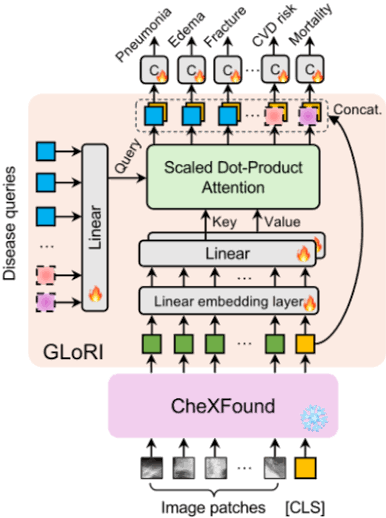
\includegraphics[width=\linewidth]{assets/vit-1.png}
	\caption{Modular schematic layout detailing parameter extraction, input token construction, and feature routing pathways between the frozen base model and the target task head.}
	\label{fig:chexfound_placeholder}
\end{figure}